% Copyright © 2012 Martin Ueding <dev@martin-ueding.de>
%
\documentclass[11pt, ngerman, fleqn]{article}

\usepackage[a4paper, left=3cm, right=2cm, top=2cm, bottom=2cm]{geometry}
\usepackage[activate]{pdfcprot}
\usepackage[thinspace, squaren]{SIunits}
\usepackage[iso]{isodate}
\usepackage[parfill]{parskip}
\usepackage[T1]{fontenc}
\usepackage[utf8]{inputenc}
\usepackage{amsmath}
\usepackage{amsthm}
\usepackage{babel}
\usepackage{color}
\usepackage{lastpage}
\usepackage{commath}
\usepackage{epstopdf}
\usepackage{fancyhdr}
\usepackage{graphicx}
\usepackage{hyperref}
\usepackage{setspace}
\usepackage{tikz}

\usepackage[charter, greekuppercase=italicized]{mathdesign}

\usetikzlibrary{arrows}
\usetikzlibrary{intersections}

\definecolor{darkblue}{rgb}{0,0,.5}
\definecolor{darkgreen}{rgb}{0,.5,0}

\hypersetup{
	breaklinks=false,
	citecolor=darkgreen,
	colorlinks=true,
	linkcolor=black,
	menucolor=black,
	urlcolor=darkblue,
}

\setlength{\columnsep}{1.5cm}

\DeclareMathOperator{\arcsinh}{arsinh}
\DeclareMathOperator{\arsinh}{arsinh}
\DeclareMathOperator{\asinh}{arsinh}
\DeclareMathOperator{\card}{card}
\DeclareMathOperator{\diam}{diam}

\newcommand{\dalambert}{\mathop{{}\Box}\nolimits}
\newcommand{\divergence}[1]{\inner{\vnabla}{#1}}
\newcommand{\ee}{\mathrm e}
\newcommand{\emesswert}{\del{\messwert \pm \messwert}}
\newcommand{\e}[1]{\cdot 10^{#1}}
\newcommand{\fehlt}{\textcolor{red}{Hier fehlen noch Inhalte.}}
\newcommand{\half}{\frac 12}
\newcommand{\ii}{\mathrm i}
\newcommand{\inner}[2]{\left\langle #1, #2 \right\rangle}
\newcommand{\laplace}{\mathop{{}\bigtriangleup}\nolimits}
\newcommand{\messwert}{\textcolor{blue}{\square}}
\newcommand{\punkte}{\textcolor{white}{xxxxxxx}}
\newcommand{\tens}[1]{\boldsymbol{\mathsf{#1}}}
\newcommand{\vnabla}{\vec \nabla}
\renewcommand{\vec}[1]{\boldsymbol{#1}}

\newcommand{\themodul}{physik311}
\newcommand{\thegruppe}{Gruppe 3 -- Matthias Rehberger}
\newcommand{\theuebung}{5}

\pagestyle{fancy}

\fancyfoot[C]{\footnotesize{\thegruppe}}
\fancyfoot[L]{\footnotesize{Martin Ueding}}
\fancyfoot[R]{\footnotesize{Seite \thepage\ / \pageref{LastPage}}}
\fancyhead[L]{\themodul{} -- Übung \theuebung}

\setcounter{section}{19}

\def\thesubsection{\thesection\alph{subsection}}

\title{\themodul{} -- Übung \theuebung \\ \vspace{0.5cm} \large{\thegruppe}}

\author{Martin Ueding \\ \small{\href{mailto:mu@uni-bonn.de}{mu@uni-bonn.de}}}

\begin{document}

\maketitle

\begin{table}[h]
	\centering
	\begin{tabular}{l|c|c|c|c|c}
		Aufgabe & \ref{1} & \ref{2} & \ref{3} & \ref{4} & $\sum$   \\
		\hline
		Punkte & \punkte & \punkte & \punkte & \punkte & \punkte
	\end{tabular}
\end{table}

%%%%%%%%%%%%%%%%%%%%%%%%%%%%%%%%%%%%%%%%%%%%%%%%%%%%%%%%%%%%%%%%%%%%%%%%%%%%%%%
%                   Hauptebenen einer gebogenen Glasscheibe                   %
%%%%%%%%%%%%%%%%%%%%%%%%%%%%%%%%%%%%%%%%%%%%%%%%%%%%%%%%%%%%%%%%%%%%%%%%%%%%%%%

\section{Hauptebenen einer gebogenen Glasscheibe}
\label 1

Sei $r:= \unit{0.1}\meter$. Die benötigen Matrizen sind:
\[
	\tens A = \begin{pmatrix}
		1 & 0 \\ \frac{n_1-n_2}{n_2 r} & \frac{n_1}{n_2}
	\end{pmatrix}
	, \quad
	\tens B = \begin{pmatrix}
		1 & 0 \\ \frac{n_1-n_2}{n_1 r} & \frac{n_2}{n_1}
	\end{pmatrix}
\]

Wenn ich einfach nur $\tens B \tens A$ rechne, erhalte ich:
\[
	\begin{pmatrix}
		1 & 0 \\ \unit{-10}{\reciprocal \meter} & 1
	\end{pmatrix}
\]

Somit wäre die Brennweite $f = \unit{0.1}\meter$.

Wenn ich den Abstand zwischen den Linsen mit einberechne, kommt allerdings
etwas anderes heraus. Da die Matrizen nur linear sind, muss ich den
horizontalen Lichtweg $w := \sqrt{d^2-h^2}$, wobei $h$ der Abstand von der
optischen Achse ist, um $h = 0$ entwickeln und erhalte nur $d$. Mit der Matrix $\tens C$
\[
	\tens C = \begin{pmatrix}
		1 & d \\ 0 & 1
	\end{pmatrix}
\]

Erhalte ich:
\[
	\tens B \tens C \tens A = \begin{pmatrix}
		0.991667 & \unit{0.00166667}{\meter} \\ \unit{- 9.95833}{\reciprocal \meter} & 0.991667
	\end{pmatrix}
\]

Dies ist dann keine normale Linse mehr, allerdings auch sehr nach an $f =
\unit{0,1}\meter$ dran.

%%%%%%%%%%%%%%%%%%%%%%%%%%%%%%%%%%%%%%%%%%%%%%%%%%%%%%%%%%%%%%%%%%%%%%%%%%%%%%%
%                            keplersches Fernrohr                             %
%%%%%%%%%%%%%%%%%%%%%%%%%%%%%%%%%%%%%%%%%%%%%%%%%%%%%%%%%%%%%%%%%%%%%%%%%%%%%%%

\section{keplersches Fernrohr}
\label 2

%%%%%%%%%%%%%%%%%%%%%%%%%%%%%%%%%%%%%%%%%%%%%%%%%%%%%%%%%%%%%%%%%%%%%%%%%%%%%%%
%                              Bildkonstruktion                               %
%%%%%%%%%%%%%%%%%%%%%%%%%%%%%%%%%%%%%%%%%%%%%%%%%%%%%%%%%%%%%%%%%%%%%%%%%%%%%%%

\section{Bildkonstruktion}
\label 3

Da die Linsen zu nah beieinander stehen, entsteht kein Bild, siehe Abbildung
\ref{fig:b}.

\begin{figure}
	\centering
	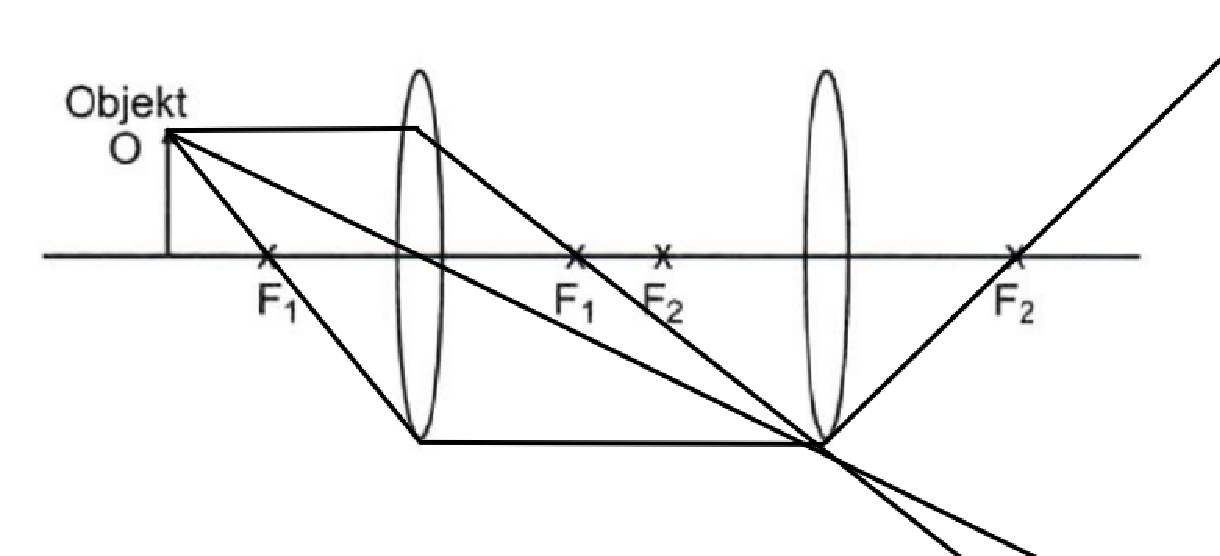
\includegraphics[width=0.6\textwidth]{Bildkonstruktion.pdf}
	\caption{Zeichnung zu Aufgabe \ref 3}
	\label{fig:b}
\end{figure}

%%%%%%%%%%%%%%%%%%%%%%%%%%%%%%%%%%%%%%%%%%%%%%%%%%%%%%%%%%%%%%%%%%%%%%%%%%%%%%%
%                               Linsenabbildung                               %
%%%%%%%%%%%%%%%%%%%%%%%%%%%%%%%%%%%%%%%%%%%%%%%%%%%%%%%%%%%%%%%%%%%%%%%%%%%%%%%

\section{Linsenabbildung}
\label 4


Es gilt

\begin{equation}
\label{GBgb}
\frac{G}{B} = \frac{g}{b}.
\end{equation}

Betrachtet man den rechten Teil zwischen Linse und Bild, findet man dort ebenfalls zwei ähnliche Dreiecke. Aus dem Strahlensatz kann man ablesen:
\begin{align*}
\frac{f}{b-f} &= \frac{G}{B} \\
%
\intertext{Zusammen mit \eqref{GBgb} ergibt sich:}
%
\frac{f}{b-f} &= \frac{g}{b} \\
bf &= bg-gf \\
bf+gf &= bg \\
f(b+g) &= bg \\
%
\intertext{Aus der Definition von $a = b + g$ folgt:}
%
fa &= bg \\
f &= \frac{bg}{a} \\
%
\intertext{Erneute Anwendung der Definition $a = b + g$:}
%
f &= \frac{(a-g)g}{a} \\
f &= \frac{ag-g^2}{a} \\
f &= g - \frac{g^2}{a} \\
%
\intertext{Einsetzen der Bedingung $a > 4f$.}
%
f &= g - \frac{g^2}{a} < g - \frac{g^2}{4f} \\
4f^2 &< 4fg - g^2 \\
4f^2 - 4fg + g^2 &< 0 \\
\left(f-\half g \right)^2 &< 0
\end{align*}

Somit gibt es genau eine Lösung für die Brennweite für den Fall $a = 4f$.

Bleiben die weiteren Fälle. Dafür wird die Banklänge in $a = r \cdot 4f$ angegeben.
\begin{align*}
f &< g - \frac{g^2}{4fr} \\
4f^2r - 4fgr + g^2 &< 0 \\
f^2 - fg + \frac{g^2}{4r} &< 0 \\
f &= \half g \pm \sqrt{\frac{1}{4} g^2 - \frac{g^2}{4r}} \\
f &= \half g \pm \half g \sqrt{1 - \frac{1}{r}}
\end{align*}

Damit es genau zwei Lösungen gibt, muss der Radikant positiv sein.
\begin{align*}
1 - \frac{1}{r} &> 0 \\
1 &> \frac{1}{r} \\
1 &< r
\end{align*}

$r$ muss also größer als 1 sein, damit es genau zwei Lösungen gibt. Für $a > 4f$ ist dies erfüllt, somit hat dieser Fall genau zwei Lösungen. Für eine Linse mit gegebener Brennweite gibt es also an zwei Stellen eine Position, wo diese Brennweite ein scharfes Bild erzeugt.


Im Grenzfall ist $a = 4f$ und das $g$ eindeutig bestimmt. Da man jedoch $g$ und $b$ vertauschen darf, müssen diese gleich sein. Es folgt $g = b = 2f$. Somit ist $\frac{g}{b}$, der Abbildungsmaßstab, 1.


%\bibliography{../../zentrale_BibTeX/Central}
%\bibliographystyle{plain}

\end{document}

% vim: spell spelllang=de
